%!TEX encoding = UTF-8 Unicode

%----------------------------------------------------------------------------------------
%	CHAPTER 4
%----------------------------------------------------------------------------------------
\newcommand\rd{\mathrm d}
\chapterimage{chapter_head_1.pdf} % Chapter heading image

\chapter[框架/体系]{The Framework 框架/体系}\label{chap4}
这一章的基本思路是,我们要在尽可能少的使用{\it 某些东西}的前提下,得到正确的关于自然的方程。{\it 某些东西}是什么?有一件事是确定的:它不应该在 Lorentz 变换下改变,否则我们会在不同的参考系下得到不同的自然规律。在数学意义上,它意味着我们寻找的这个东西是个标量,依照洛伦兹群的 \( (0,0) \) 表示作变换。再考虑到自然总依简单而行,我们已经足够导出关于自然的方程了。

从这个想法出发,我们将会引入{\bf 拉格朗日形式(Lagrangian formalism)}。通过极小化理论的中心对象,我们可以得到用以描述问题中的物理系统的运动方程。极小化过程的结果被称作 {\bf Euler-Lagrange 方程}。

通过拉格朗日形式,我们可以得到物理中最重要的定理:Noether 定理。这个定理揭示了对称性和守恒量%
\mpar{守恒量指的是不随时间变化的物理量。例如一个给定体系的能量或动量。数学上意味着\(\partial_t Q = 0 \rightarrow Q = \text{常数}\)。}%
之间的深刻联系。我们将在下一章中利用它来理解,理论是如何来描述实验测量量的。

\section[拉格朗日形式]{Lagrangian Formalism \quad 拉格朗日形式}\label{sec4.1}

拉格朗日形式是在基础物理中被广泛运用的一个强有力的框架%
\mpar{物理中当然有其他框架,例如以{\bf 哈密顿量(Hamiltonian)}为中心对象的{\bf 哈密顿形式(Hamiltonian formalism)}。哈密顿量的问题在于它不是洛伦兹不变的,因为它所代表的能量,仅仅是{\bf 四动量(covariant energy-impulse vector)}的一个分量}%
。由于理论的基本对象--{\bf 拉格朗日量(Lagrangian)}是一个标量%
\mpar{标量指依照洛伦兹群的 \( (0,0) \) 表示作变换的对象。这意味着它不在洛伦兹变换下改变}%
,它相对简单。如果你希望从对称性的观点考虑问题,这种形式将会是非常有用的。如果我们要求拉格朗日量的积分,{\bf 作用量(action)},在某些对称变换下不变,我们即要求体系的动力学遵从该对称性。

\subsection{Fermat 原理}\label{sec4.1.1}
\begin{quote}
Whenever any action occurs in nature, the quantity of action employed by this change is the least possible.\\
- Pierre de Maupertius \mpar{Recherche des loix du mouvement (1746)}
\end{quote}

拉格朗日形式的思想源于 Fermat 原理:光在两空间点间传播总依耗时最短的路径\(q(t)\)而行。数学上来讲,如果我们定义给定路径\(q(t)\)的作用量为
\[
S_{\text{light}}[{\mathbf q}(t)] = \int ~{\mathrm d}t
\]
而我们的任务便是找到一条特定的路径\(q(t)\)使作用量取极小值%
\mpar{此处的作用量仅仅是沿给定路径对时间的积分,但一般而言作用量会更加复杂,我们待会儿就能见到}%
为了得到一个给定{\bf 函数}的极小值%
\mpar{一般而言,我们希望找到{\bf 极值(extremums)},即极小值{\bf 和}极大值。下一节中的方法足以找到这两者。无论如何,我们将继续谈论极小值}%
,我们可以求得其导函数并令其为零;而为了找到{\bf 泛函}\(S[q(t)]\)——函数\(q(t)\)的函数\(S\)——的极小值,就得要一个新的数学工具:{\bf 变分法}。

\marginpar{
	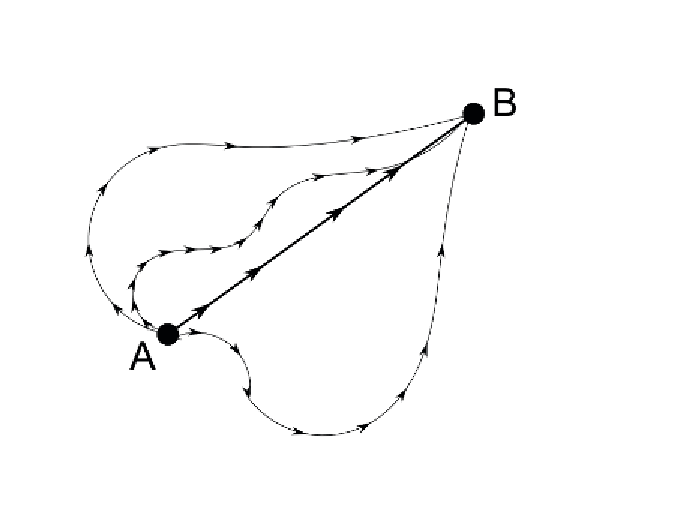
\includegraphics[scale=0.35]{./Figure/fig4_1} 
	\figcaption{对于给定初末端点的路径的扰动}
}

\subsection{变分法:基本思想}\label{sec4.1.2}

在思考如何发展一套能够找到泛函极值的新理论之前,我们需要倒回去想想什么给出一个数学上的极小点。变分法给出的答案是,极小点由极小点邻域的性质决定。例如,让我们尝试寻找一个寻常函数\(f(x)=3x^2+x\)的极小点\(x_{\min}\)。我们从一个特定点\(x=a\)出发,仔细考察其邻域。数学上它意味着\(a + \epsilon\),其中\(\epsilon\)代表无穷小量(可正可负)。我们将\(a\)的变分代入函数\(f(x)\):
\[
f(a+\epsilon) = 3(a+\epsilon)^2+(a+\epsilon) = 3(a^2+2a\epsilon+\epsilon^2)+a+\epsilon \text{。}
\]
如果\(a\)是极小点,\(\epsilon\)的一阶变分必需为零,否则我们可以取\(\epsilon\)为负\(\epsilon < 0\),这样\(f(a+\epsilon)\)就会比\(f(a)\)更小%
\footnote{\textcolor{red}{译注:此处讨论有误}}%
。因此,我们将线性依赖于\(\epsilon\)的项取出并令其为零。
\[
3 \cdot 2a\epsilon + \epsilon \overset{\text{!}}{=} 0 \rightarrow 6a+1\overset{\text{!}}{=}0\text{。}
\]
由此我们找到极小点
\[
x_{\min} = a = -\frac{1}{6} \text{,}
\]
它自然和我们求导\(f(x)=3x^2+x\leftarrow f'(x)=6x+1\)并令其为零的办法得到的结果一致。对于寻常函数而言,这只是一个用来干同一件事不同方法而已%
\footnote{译注:对于受微元法茶毒的物竞生而言,求导才是用来干这件事的不同方法。}%
,但是变分法却能找到泛函的极值点。我们马上就能看到,应当如何处理一个一般的作用量泛函。

拉格朗日形式的中心思想在于对于有质量的物体,也存在一个与对光的 Fermat 原理相类似的原理。当然,它不可能直接遵从费马原理,但是我们可以从一个更一般的形式出发
\[
S[q(t)]=\int {\mathcal L}~{\mathrm d}t
\]
其中\(\mathcal L\)一般是一个非常数的参量,被称为拉格朗日量。对于光而言,这个参量是个常数。一般的,拉格朗日量依赖于物体的坐标和速度\({\mathcal L}={\mathcal L}(q(t),\frac{\partial}{\partial t} q(t))\)。在下一节中我们将仔细讨论这件事%
\mpar{我们的任务是找到对于给定拉格朗日量和初始条件有着最小作用量的路径\(q(t)\)。在此之前,我们得先找到正确的拉格朗日量,用以描述问题中的物理系统。这是我们在上一章中所讨论的对称性所能发挥作用的地方。通过要求拉格朗日量在洛伦兹群的所有变换下不变,我们就能找到正确的拉格朗日量}%
。在仔细讨论如何对这样一个泛函使用变分法之前,我们需要先讲讲两个小问题。

\section[限制]{Restrictions \quad 限制}\label{sec4.2}
正如我们在\ref{sec1.1}节中所提到的,现有理论中有一些限制条件是无法从第一性原理中得到的。我们所能知道是,如果想得到一个有意义的理论,我们必须加上这些限制。

一个重要的限制是,我们仅允许拉格朗日量中出现尽可能低阶的非平凡%
\footnote{译注:Non-trival. Trival 这个词常包含简单、弱智、无意义之义。}%
导数。这里平凡指的是对于系统的动力学,即运动方程,没有影响。某些理论会包含一阶导数,另外一些带二阶导数。一个给定理论所含的最低阶导数由该条件决定:拉格朗日量在 Lorentz 变换下不变%
\mpar{实际上,作用量才应该是 Lorentz 不变的。但如果拉格朗日量满足这个条件,那作用量自然也是。}%
,否则我们将在不同的参考系下导出不同的运动方程%
\footnote{\textcolor{red}{译注:此处讨论疑有误,作者此前并没有说明积分中的时间是坐标时还是固有时}}%
。对于某些理论,我们无法写出一个仅含一阶导数项的不变量,那么此时二阶导数便成了最低阶导数项。

我们并不清楚如何处理包含高阶导数的理论,它们有一些根本的困难%
\mpar{这些困难包括 Ostrogradski 不稳定性,即包含高阶导数的系统的能量没有下界,以至于系统中的所有态总会自发衰变到能量更低的态上去。这类系统中找不到稳定的状态。}%
。另外,拉格朗日量中的高阶导数会使得运动方程中也包含高阶导数,这样我们必须知道更多的初始条件才能决定物体的运动。

有些人会宣称对理论所包含导数阶数的限制源于我们希望得到一个局域%
\mpar{局域性是狭义相对论的基本假定,\ref{sec2.4}已作阐述}%
理论,但这个要求仅会排除掉那些无穷阶导数。一个非局域相互作用有如下形式%
\mpar{我们将会讨论粒子的拉格朗日理论:寻求粒子的路径;也会讨论场的拉格朗日理论:寻求场函数\(\phi(x)\)。这将是下一节的主题。}
\begin{equation}
\Phi(x-h)\Phi(x)
\end{equation}
即,时空中距离为\(h\)的两个点的场相互作用。利用 Taylor 展开我们有%
\footnote{\textcolor{red}{译注:此式有误}}
\begin{equation}
\Phi(x-h) = \sum\limits_{k=0}^{\infty}\left(\left(\frac{\partial}{\partial x}\right)^k\left.\Phi(x)\right|_{x=h}\right) \frac{(x-h)^k}{k!}
\end{equation}
即包含无穷阶导数会导致一个非局域的理论。

另外一个限制是,要得到一个自由(无相互作用)场/粒子的理论,我们只能写到二次项。这意味着我们只会考虑%
\mpar{从另外一个角度来看,这再次表示我们只引入最低阶的非平凡项。我们随后就会看到,含\(\Phi^0\)和\(\Phi^1\)的项是平凡的,因此我们这次用的是\(\Phi\)的最低阶非平凡项}
\[
\Phi^0, \Phi^1, \Phi^2
\]
这样的项。例如,形如\(\Phi^2 \partial_\mu \Phi\)的项是\(\Phi\)的三阶项,因而不会被包含在我们自由理论的拉格朗日量中。

\section[粒子理论与场论]{Particle Theories vs. Field Theories \quad 粒子理论与场论}\label{sec4.3}
我们目前有两套用以描述自然的理论框架。一套是粒子理论,用依赖于时间的粒子位置描述物理系统,即\(\vec{q}=\vec{q}(t)\)。由于我们不是非得在使用笛卡尔坐标系%
\mpar{例如,我们可以用球坐标系}%
,所以用的是字母\(q\)而不是\(x\)。对于这样的理论,拉格朗日量依赖于坐标\(\vec{q}\),速度\(\partial_t\vec{q}\)和时间\(t\):%
\footnote{译注:严格说来,依赖于坐标函数\(\vec{q}(t)\),速度函数\(\partial_t\vec{q}(t)\)和时间\(t\)}
\begin{equation}
{\mathcal L} = {\mathcal L} (\vec{q},\partial_t\vec{q},t)
\end{equation}

一个著名的例子是这个能导出经典力学的牛顿运动方程的拉格朗日量\({\mathcal L} = \frac{1}{2}m\vec{q}^2\)。我们将在稍后进行相当详细的讨论。

另一套是场论:使用场而不是独立粒子的坐标来描述自然%
\mpar{量子场论有一个特别优美的性质是关于如何将粒子引进的。我们将在\ref{chap6}中看到场有能力产生和湮灭粒子}%
。在这套理论中,时空构成了场\(\Phi(\vec{x},t)\)表演的舞台。利用前面提到过的限制,我们得到%
\mpar{这里我故意使用了不同的符号\({\mathscr L}\),因为在场论中大多数时候我们都在和拉格朗日量密度\({\mathscr L}\)打交道。两者之间满足关系式\({\mathcal L} = \int{\mathrm d}^3\bm{x}~{\mathscr L}\)}
\begin{equation}
{\mathscr L} = {\mathscr L} (\Phi(\vec{x},t), \partial_\mu \Phi(\vec{x},t), \vec{x})
\end{equation}

一个著名的例子是我们将用以导出 Klein-Gordon 方程的拉格朗日量\({\mathscr L} = \frac{1}{2}\left(\partial_\mu\Phi\partial^\mu\Phi-m^2\Phi^2\right)\)。

场论的一大优点是它将时空等价的对待。在粒子理论中我们使用空间坐标\(\vec{q}(t)\)作为时间的函数来描述我们的粒子。尤其是,拉格朗日量中没有类似于\(\partial_{\vec{q}}t\)的项(如果出现了这类项,我们该怎样理解它呢?)当我们讨论粒子的坐标时,意义是清楚的,但对时间做类似的陈述时,却很难有明确的意义%
\footnote{译注:利用不那么古老的相对论性语言,粒子理论下时空坐标是可以在形式上被同等对待的:用以求导的东西只能是曲线的参数,它可以取作粒子世界线的固有时、某一坐标系的坐标时、或者其他什么东西(只要性质合适,也可以是空间坐标);而时空坐标则被同样的求导。}。

讨论了这么多,我们终于可以回到这章开头所说的极小化问题上来了。我们希望找到某些泛函
\[
S[q(t)] = \int {\mathcal L}~{\mathrm d}t
\]
的极小值,以得到正确的运动方程。

对于粒子而言,方程的解是使得泛函取极小值的正确路径;而对于场而言,解是正确的场函数。

此刻请不用担心\(\mathcal L\)的具体形式,在下面数章中我们将详细讨论如何对问题中的系统导出正确的拉格朗日量\(L\)。现在,我们将使用之前所介绍过的变分法,对于一个一般的\(\mathcal L\)导出泛函\(S[q(t)]\)的极小值。极小化过程将给出系统的运动方程。

\section[欧拉-拉格朗日方程]{Euler-Lagrange equation \quad 欧拉-拉格朗日方程}\label{sec4.4}
我们从粒子理论出发,它能让我们搞清楚,在给定初末点后,粒子是如何运动的。数学上,我们需要找到{\bf 函数}\(q(t)\)使得作用量\footnote{此处原文字体有误}
\[
S = \int_{t_1}^{t_2} {\mathcal L}\left(q(t),\frac{\rd q(t)}{\rd t},t\right)
\]
取得其极值(极大值或极小值)。

我们使用记号
\[
\dot q(t) = \frac{\rd q(t)}{\rd t}\text{。}
\]
与之前的例子类似,取\(q(t)=a(t)\)并让对这个函数进行一个扰动
\[
a(t) + \epsilon(t)
\]
其中\(\epsilon\)依旧是一个无穷小量。对于一个粒子而言,我们必须同时改变其速度\(\dot a(t) + \dot\epsilon(t)\),其中\(\dot\epsilon(t) = \frac{\rd \epsilon(t)}{\rd t}\)。

在边界上,变换后的路径应与原路径相同:
\begin{equation}
0 = \epsilon(t_1) = \epsilon(t_2)
\label{eq:4.5}
\end{equation}
这是因为我们寻找的是使作用量积分取极值的{\bf 给定初末端点}的路径。

这个扰动使得泛函变为
\[
S = \int_{t_1}^{t_2} {\mathcal L}\left(q+\epsilon,\dot q + \dot \epsilon, t\right)~\rd t \text{。}
\]
与之前的例子类似,当我们寻求极小值时,我们要求线性依赖于扰动\(\epsilon\)的项为零。由于我们处理的是一个一般性的\(\mathcal L\),故将其展开成泰勒级数%
\mpar{我们正使用的是这个公式的多变量形式,参见附录\ref{appendix2.3}:
\[
\begin{aligned}
{\mathcal L}\left(q+\epsilon,\dot q + \dot \epsilon, t\right) = {\mathcal L}(q,\dot q,t) + \\
\epsilon\frac{\partial \mathcal{L}}{\partial q} + \dot\epsilon\frac{\partial \mathcal{L}}{\partial \dot q} + \dots
\end{aligned}
\]}%对原文公式有改动
,并令一阶项为零
\begin{equation}
\int_{t_1}^{t_2} \rd t ~ \left[ \epsilon(t) \frac{\partial \mathcal{L}}{\partial q} + \left( \frac{\rd}{\rd t} \epsilon(t) \right)\frac{\partial \mathcal{L}}{\partial \dot q} \right] \overset{\text{!}}{=} 0 \text{。}
\label{eq:4.6}
\end{equation}
对后一项做分部积分%
\mpar{分部积分是莱布尼兹律的直接推论,详见附录\ref{appendix2.3}}%
得到
\[
\begin{aligned}
\int_{t_1}^{t_2} \rd t ~ \left( \frac{\rd}{\rd t} \epsilon(t) \right)\frac{\partial \mathcal{L}(q,\dot q,t)}{\partial \dot q} =\\
\left.\epsilon(t)\frac{\partial \mathcal{L}(q,\dot q,t)}{\partial \dot q}\right|_{t_1}^{t_2} - \int_{t_1}^{t_2} \rd t ~  \epsilon(t) \frac{\rd}{\rd t} \left( \frac{\partial \mathcal{L}(q,\dot q,t)}{\partial \dot q} \right)
\end{aligned}
\]
利用\ref{eq:4.5}式有
\[
\left.\epsilon(t)\frac{\partial \mathcal{L}(q,\dot q,t)}{\partial \dot q}\right|_{t_1}^{t_2} = 0
\]
因此,我们可以将\ref{eq:4.6}改写为
\[
\int_{t_1}^{t_2} \rd t ~\epsilon(t) \left[ \frac{\partial \mathcal{L}}{\partial q} - \frac{\rd}{\rd t} \left( \frac{\partial \mathcal{L}(q,\dot q,t)}{\partial \dot q}\right) \right] \overset{\text{!}}{=} 0
\]
易见上式对于任意扰动\(\epsilon(t)\)为零仅当方括号\([~]\)内的表达式为零。故有%
\mpar{可能你会对于两类不同的导数符号感到困惑。\(\frac{\rd}{\rd t}\)被称作对\(t\)的全导数,而\(\frac{\partial}{\partial t}\)被称为偏导数。全导数给出总改变量,函数\(f\)的变化率,即偏导数,乘以变量自身的改变,之和。
例如,三维空间中的函数\(f(x(t),y(t),z(t))\)的总变化率为\(\frac{\rd f}{\rd t} = \frac{\partial f}{\partial x}\frac{\partial x}{\partial t}+\frac{\partial f}{\partial y}\frac{\partial y}{\partial t}+\frac{\partial f}{\partial z}\frac{\partial z}{\partial t}\)。
即变化率乘以自身的改变量。
相对的,偏导数仅给出总改变量的一部分。对于一个不显式的依赖于\(t\)的函数,其偏导数为零。例如,对于\(f(x(t),y(t))=x^2y+y^3\),我们有\(\frac{\partial f}{\partial t}=0\),但\(\frac{\partial f}{\partial x}=2xy \ne 0, \frac{\partial f}{\partial y}=x^2+3y^2 \ne 0\)。
因此\(\frac{\rd f}{\rd t}=2xy\frac{\partial x}{\partial t}+(x^2+3y^2)\frac{\partial y}{\partial t}\)。
作为对比,对于另一个函数\(g(x(t),y(t),t)=x^2t+y\)我们有\(\frac{\partial g}{\partial t}=x^2\)
}
\begin{equation}
\frac{\partial \mathcal{L}}{\partial q} - \frac{\rd}{\rd t} \left( \frac{\partial \mathcal{L}(q,\dot q,t)}{\partial \dot q} \right)= 0
\label{eq:4.7}
\end{equation}
这就是著名的{\bf 欧拉-拉格朗日方程(Euler-Lagrange equation)}

我们可以用类似的办法处理场论。首先,注意到我们需要将时空同等对待。因此我们引入拉格朗日量密度:
\begin{equation}
{\mathcal L} = \int{\mathrm d}^3\bm{x}~{\mathscr L}(\Phi^i,\partial_\mu \Phi^i) 
\end{equation}
并用拉格朗日量密度来表示作用量
\begin{equation}
S = \int \rd t~{\mathcal L} = \int{\mathrm d}^4\bm{x}~{\mathscr L}(\Phi^i,\partial_\mu \Phi^i) 
\end{equation}
依照上面讲过的步骤,我们可以得到场的运动方程组%
\mpar{在这里用“组”字是因为对于每一个场分量\(\Phi_1,\Phi_2,\dots\)我们都可以得到一个方程}%
:
\begin{equation}
\frac{\partial \mathcal{L}}{\partial \Phi} - \partial_\mu \left( \frac{\partial \mathcal{L}}{\partial (\partial_\mu \Phi)} \right)= 0
\end{equation}

在下一章中我们将用拉格朗日形式导出近代物理学中重要的一个定理。借助其我们能看到对称性与守恒量之间的深刻联系。守恒量是描述自然的合适参量%
\mpar{我们将其视做锚定这个复杂的世界之物。不论万事万物如何改变,守恒量依旧是守恒量。}%
,从这个定理中我们将学会如何和它打交道。

\section[Noether 定理]{Noether's Theorem \quad Noether 定理}\label{sec4.5}
Noether 定理表示,拉格朗日量的每一个对称性都对应于一个守恒量。换言之,物理学家用于描述自然(守恒量)的记号和对称性直接相关。这确实是科学史上最美的创见之一。

\subsection{粒子理论的Noether 定理}\label{sec4.5.1}
让我们先看看能对粒子理论中的守恒量做点什么。我们将局限于连续对称性,由此我们能使用无穷小变换。如同前面数章所言,我们可以通过重复无穷小变换来得到一个有限的变换。拉格朗日量在无穷小变换%
\mpar{用符号\(\delta\)来表述小扰动,大概不会和用来表述偏导数的\(\partial\)相混淆}%
\(q\rightarrow q'=q+\delta q\)下不变的性质用数学表述如下%
\footnote{译者注:该书中$\delta S$,$\delta {\mathcal L}$与平常的约定都差了一个负号。}
\begin{equation}
\begin{aligned}
\delta {\mathcal L} &= {\mathcal L}(q,\frac{\rd q}{\rd t},t) - {\mathcal L}(q+\delta q,\frac{\rd (q+\delta q)}{\rd t},t) \\
&= {\mathcal L}(q,\frac{\rd q}{\rd t},t) - {\mathcal L}(q+\delta q,\frac{\rd q}{\rd t}+\frac{\rd \delta q}{\rd t},t) \overset{\text{!}}{=} 0 
\end{aligned}
\label{eq:4.11}
\end{equation}

要求拉格朗日量是变换不变的,这个条件太强了。为了保证动力学一样,不变的应该是作用量而不是拉格朗日量。当然,如果拉格朗日量不变,作用量自然不变:
\begin{equation}
\delta S = \int \rd t~{\mathcal L}(q,\frac{\rd q}{\rd t},t) -  \int \rd t~{\mathcal L}(q+\delta q,\frac{\rd q}{\rd t},t) = \int \rd t~\delta{\mathcal L}\underbrace{=}_{\mathclap{\text{若}~\delta{\mathcal L}=0}} 0
\end{equation}
在什么情况下,拉格朗日量改变而作用量不变呢?答案是,给拉格朗日量加上一个任意函数$G$对时间的全导数
\[
{\mathcal L}\rightarrow{\mathcal L}+\frac{\rd G}{\rd t}
\]
这时作用量不变%
\mpar{用到了$\delta G =\frac{\partial G}{\partial q}\delta q$。这是因为$G=G(q)$而我们改变了$q$,故$G$的扰动等于改变率$\frac{\partial G}{\partial q}$乘上$q$的扰动}
\[
\delta S \rightarrow \delta S' = \delta S + \int_{t_1}^{t_2} {\rd t~\frac{\rd}{\rd t}\delta G} = \delta S + \underbrace{\left.\frac{\partial G}{\partial q} \delta q \right|_{t_1}^{t_2}}_{\mathclap{=0~\text{因为}~\delta q(t_1)=\delta q(t_2)=0}}.
\]
在最后一步中,我们用到了扰动$\delta q$在初末时刻$(t_1,t_2)$为零。由此我们可知,我们并不需要去强求拉格朗日量的扰动$\delta {\mathcal L}$为零,而仅需满足一个更弱的条件
\begin{equation}
\delta {\mathcal L} \overset{\text{!}}{=} \frac{\rd G}{\rd t}.
\end{equation}

这意味着拉格朗日量可以在不改变作用量和运动方程的情况下,加减某个函数的全微分$\frac{\rd G}{\rd t}$。将\ref{eq:4.11}式的右端由$0$改作$\frac{\rd G}{\rd t}$,我们有
\begin{equation}
\delta {\mathcal L} =  {\mathcal L}(q,\frac{\rd q}{\rd t},t) - {\mathcal L}(q+\delta q,\frac{\rd q}{\rd t}+\frac{\rd (\delta q)}{\rd t},t) \overset{\text{!}}{=} \frac{\rd G}{\rd t} 
\end{equation}
将第二项按 Taylor 级数展开到$\delta q$的一阶项,并使用记号$\frac{\rd q}{\rd t}=\dot q$
\begin{equation}
\begin{aligned}
&\rightarrow \delta {\mathcal L} =  {\mathcal L} - {\mathcal L} -\frac{\partial \mathcal L}{\partial q} \delta q - \frac{\partial \mathcal L}{\partial \dot q} \delta \dot q \overset{\text{!}}{=} \frac{\rd G}{\rd t}  \\
&\rightarrow \delta {\mathcal L} =  -\frac{\partial \mathcal L}{\partial q} \delta q - \frac{\partial \mathcal L}{\partial \dot q} \delta \dot q \overset{\text{!}}{=} \frac{\rd G}{\rd t}
\end{aligned}
\label{eq:4.15}
\end{equation}
利用欧拉-拉格朗日方程\mpar{\ref{eq:4.7}式:$\frac{\partial \mathcal L}{\partial q} = \frac{\rd}{\rd t} \left(\frac{\partial \mathcal L}{\partial \dot q}\right)$}重写\ref{eq:4.15}式,有
\[
\rightarrow \delta {\mathcal L} =  -\frac{\rd}{\rd t} \left(\frac{\partial \mathcal L}{\partial \dot q}\right) \delta q - \frac{\partial \mathcal L}{\partial \dot q} \delta \dot q \overset{\text{!}}{=} \frac{\rd G}{\rd t}
\]
利用莱布尼兹律\mpar{如果你对莱布尼兹律仍有疑问,请参考\ref{appendenix2.1}},我们有
\begin{equation}
\begin{aligned}
&\rightarrow \delta {\mathcal L} =  -\frac{\rd}{\rd t} \left(\frac{\partial \mathcal L}{\partial \dot q}\delta q\right) \overset{\text{!}}{=} \frac{\rd G}{\rd t} \\
&\rightarrow\frac{\rd}{\rd t} \underbrace{\left(\frac{\partial \mathcal L}{\partial \dot q}\delta q + G\right)}_{\equiv J} \overset{\text{!}}{=} 0
\end{aligned}
\end{equation}
由此我们得到了一个不随时间变化的物理量$J$:
\begin{equation}
J = \frac{\partial \mathcal L}{\partial \dot q}\delta q + G\text{,}
\end{equation}
这是因为
\[
\frac{\rd J}{\rd t} = 0 \rightarrow J = \text{常数。}
\]

为了看清楚这一点,我们先借用一下后面章节的结论:常质量自由粒子的牛顿第二定律是%
\mpar{如果$q$代表某个物体的位置,则$\frac{\rd q}{\rd t}=\dot q$是这个物体的速度,$\frac{\rd}{\rd t}\frac{\rd q}{\rd t}=\frac{\rd^2 q}{\rd t^2}=\ddot q$是加速度。}
\begin{equation}
m{\ddot\vec{q}} = 0 \text{。}
\end{equation}
你可以将其代入欧拉-拉格朗日方程(\ref{eq:4.7}式)中去验证它。

